\section{Proof Strategy: Overview}\label{sec:proof-outline}
%=============================================================================

The proof uses the four-stage Jang--conformal--AMO method, extending techniques from the spacetime Penrose inequality literature \cite{braykhuri2010, hankhuri2013, amo2022}. 

\subsection{Proof Roadmap}\label{subsec:proof-roadmap}

For readers seeking a quick overview of the logical structure, the proof follows this dependency chain:

\begin{center}
\fbox{\parbox{0.92\textwidth}{
\textbf{Proof Roadmap: From Hypotheses to Conclusion}
\[
\boxed{\text{(H1) DEC}} \xrightarrow{\text{Jang eq.}} R_{\bar{g}} \geq 0 \xrightarrow{\text{AM-Lich.}} \phi > 0 \text{ exists} \xrightarrow{\text{conformal}} R_{\tilde{g}} \geq 0
\]
\[
\boxed{\text{(H2) Axisym.}} + \boxed{\text{(H3) Vacuum}} \xrightarrow{d^\dagger\alpha_J=0} J(t) = J \text{ (conserved)}
\]
\[
\boxed{\text{(H4) Stable MOTS}} \xrightarrow{\text{Dain--Reiris}} A(0) \geq 8\pi|J| \xrightarrow{A'(t)\geq 0} A(t) \geq 8\pi|J| \;\forall t
\]
\[
R_{\tilde{g}} \geq 0 + J \text{ conserved} + \text{sub-extremal} \xrightarrow{\text{AMO}} \frac{d}{dt}m_{H,J}(t) \geq 0
\]
\[
m_{H,J}(1) = M_{\text{ADM}} \geq m_{H,J}(0) = \sqrt{\frac{A}{16\pi} + \frac{4\pi J^2}{A}} \quad \checkmark
\]
}}
\end{center}

\subsection{Comparison with Prior Penrose Inequality Proofs}

The following table compares our approach with the two established proofs of the (non-rotating) Riemannian Penrose inequality:

\begin{table}[htbp]
\centering
\small
\begin{tabular}{@{}p{2.8cm}p{3.5cm}p{3.5cm}p{4cm}@{}}
\toprule
\textbf{Feature} & \textbf{Huisken--Ilmanen} \cite{huisken2001} & \textbf{Bray} \cite{bray2001} & \textbf{This Paper} \\
\midrule
Flow type & Inverse mean curvature (IMCF) & Conformal flow & $p$-harmonic (AMO) \\
Handles $J \neq 0$? & No (time-symmetric) & No (time-symmetric) & \textbf{Yes} \\
Curvature assumption & $R_g \geq 0$ & $R_g \geq 0$ & DEC + vacuum exterior \\
Boundary condition & Weak solution jumps & Horizons shrink to points & Cylindrical ends \\
Monotonic quantity & Hawking mass $m_H$ & Isoperimetric mass & AM-Hawking mass $m_{H,J}$ \\
Rigidity characterization & Schwarzschild & Schwarzschild & Kerr \\
Multiple horizons? & Yes (jumps) & Yes (conformal) & One (outermost) \\
Regularity required & Weak solutions & $C^2$ & $C^{2,\beta}$ weighted \\
\bottomrule
\end{tabular}
\caption{Comparison of Penrose inequality proof methods. The key advantage of our approach is the ability to handle rotating black holes ($J \neq 0$), at the cost of requiring stronger hypotheses (vacuum exterior, axisymmetry).}
\label{tab:proof-comparison}
\end{table}

\begin{remark}[Self-Contained Proof]
The proof is \textbf{self-contained} in that it does not require prior results about the Penrose inequality as inputs. Each stage uses established techniques from geometric analysis: Han--Khuri \cite[Theorem~1.1, Proposition~4.5]{hankhuri2013} for Jang existence, standard elliptic theory for the Lichnerowicz equation, AMO \cite[Theorem~1.1]{amo2022} for monotonicity, and Dain--Reiris \cite[Theorem~1]{dain2011} for the area-angular momentum inequality on MOTS. What is new is the synthesis of these methods and the introduction of the AM-Hawking mass for the rotating case.
\end{remark}

\subsection{The Four Stages}

The proof proceeds through four main stages, each building on the previous. We summarize the construction before presenting the technical details.

\begin{figure}[htbp]
\centering
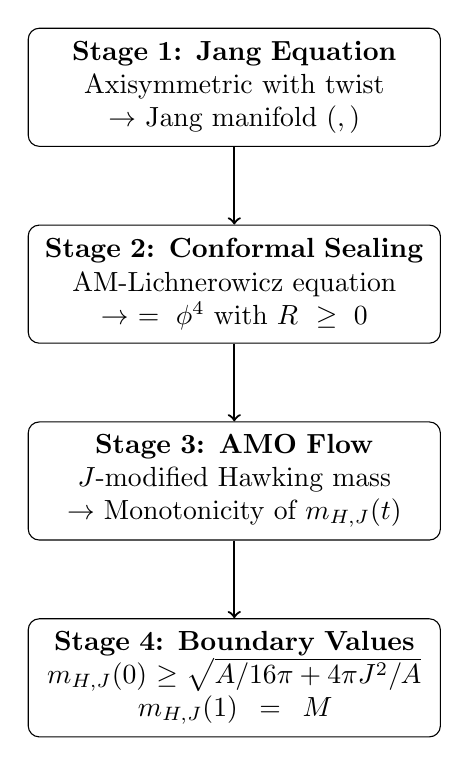
\begin{tikzpicture}[node distance=2.5cm, auto,
    block/.style={rectangle, draw, text width=5cm, text centered, rounded corners, minimum height=1.5cm}]
    
    \node[block] (stage1) {\textbf{Stage 1: Jang Equation}\\Axisymmetric with twist\\$\to$ Jang manifold $(\bM, \bg)$};
    \node[block, below of=stage1] (stage2) {\textbf{Stage 2: Conformal Sealing}\\AM-Lichnerowicz equation\\$\to$ $\tg = \phi^4 \bg$ with $R_{\tg} \geq 0$};
    \node[block, below of=stage2] (stage3) {\textbf{Stage 3: AMO Flow}\\$J$-modified Hawking mass\\$\to$ Monotonicity of $m_{H,J}(t)$};
    \node[block, below of=stage3] (stage4) {\textbf{Stage 4: Boundary Values}\\$m_{H,J}(0) \geq \sqrt{A/16\pi + 4\pi J^2/A}$\\$m_{H,J}(1) = M_{\ADM}$};
    
    \draw[->, thick] (stage1) -- (stage2);
    \draw[->, thick] (stage2) -- (stage3);
    \draw[->, thick] (stage3) -- (stage4);
\end{tikzpicture}
\caption{The four-stage Jang--conformal--AMO proof strategy. Each stage transforms the geometric data while preserving or establishing key properties needed for the inequality.}
\label{fig:four-stages}
\end{figure}

\begin{center}
\fbox{\parbox{0.95\textwidth}{
\textbf{Schematic: How the Inequality Emerges}
\begin{center}
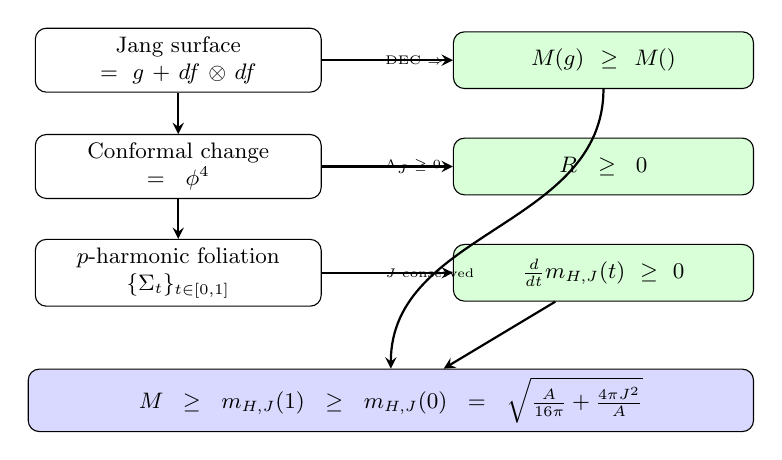
\begin{tikzpicture}[scale=0.9, transform shape,
    box/.style={rectangle, draw, rounded corners, minimum height=0.8cm, text centered, font=\small},
    ineq/.style={rectangle, draw, rounded corners, fill=green!15, minimum height=0.8cm, text centered, font=\small},
    flow/.style={->, thick, >=stealth}]
    
    % Left column: Geometric constructions
    \node[box, text width=3.8cm] (jang) at (0,4) {Jang surface\\$\bg = g + df \otimes df$};
    \node[box, text width=3.8cm] (conf) at (0,2.5) {Conformal change\\$\tg = \phi^4 \bg$};
    \node[box, text width=3.8cm] (flow) at (0,1) {$p$-harmonic foliation\\$\{\Sigma_t\}_{t\in[0,1]}$};
    
    % Right column: Key quantities
    \node[ineq, text width=4cm] (mass1) at (6,4) {$M_{\ADM}(g) \geq M_{\ADM}(\tg)$};
    \node[ineq, text width=4cm] (curv) at (6,2.5) {$R_{\tg} \geq 0$};
    \node[ineq, text width=4cm] (mono) at (6,1) {$\frac{d}{dt}m_{H,J}(t) \geq 0$};
    
    % Connecting arrows
    \draw[flow] (jang) -- (mass1);
    \draw[flow] (conf) -- (curv);
    \draw[flow] (flow) -- (mono);
    \draw[flow] (jang) -- (conf);
    \draw[flow] (conf) -- (flow);
    
    % Bottom: The final inequality
    \node[ineq, text width=10cm, fill=blue!15] (final) at (3,-0.8) {%
        $M_{\ADM} \geq m_{H,J}(1) \geq m_{H,J}(0) = \sqrt{\frac{A}{16\pi} + \frac{4\pi J^2}{A}}$};
    
    \draw[flow] (mono) -- (final);
    \draw[flow] (mass1) to[out=-90,in=90] (final);
    
    % Annotations
    \node[font=\tiny, right] at (2.8,4) {DEC $\Rightarrow$};
    \node[font=\tiny, right] at (2.8,2.5) {$\Lambda_J \geq 0$};
    \node[font=\tiny, right] at (2.8,1) {$J$ conserved};
\end{tikzpicture}
\end{center}
\textbf{Reading the diagram:} The left column shows the geometric constructions (Jang surface $\to$ conformal metric $\to$ foliation). Each construction produces a key inequality (right column). The final inequality combines mass control, curvature positivity, and monotonicity.
}}
\captionof{figure}{Schematic showing how the AM-Penrose inequality emerges from the geometric constructions.}
\label{fig:inequality-schematic}
\end{center}

\begin{figure}[htbp]
\centering
\fbox{\parbox{0.98\textwidth}{
\textbf{Manifold Transformation Chain}
\begin{center}
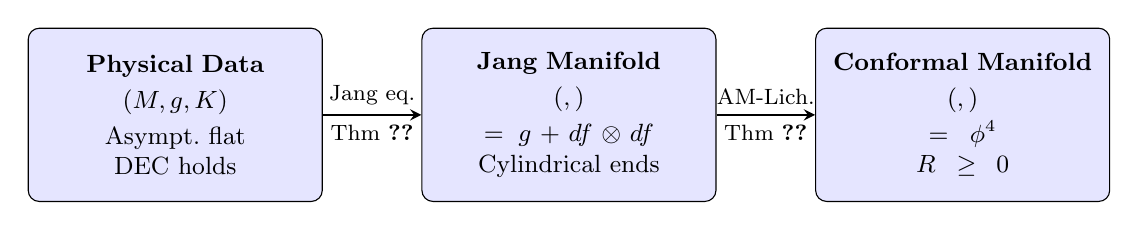
\begin{tikzpicture}[node distance=5cm, auto,
    manifold/.style={rectangle, draw, text width=3.5cm, text centered, rounded corners, minimum height=2.2cm, fill=blue!10, font=\small},
    arrow/.style={->, thick, >=stealth}]
    
    \node[manifold] (M) {\textbf{Physical Data}\\[2pt]$(M, g, K)$\\[2pt]Asympt.\ flat\\DEC holds};
    \node[manifold, right of=M] (Mbar) {\textbf{Jang Manifold}\\[2pt]$(\bM, \bg)$\\[2pt]$\bg = g + df\otimes df$\\Cylindrical ends};
    \node[manifold, right of=Mbar] (Mtilde) {\textbf{Conformal Manifold}\\[2pt]$(\tM, \tg)$\\[2pt]$\tg = \phi^4\bg$\\$R_{\tg} \geq 0$};
    
    \draw[arrow] (M) -- node[above, font=\footnotesize] {Jang eq.} node[below, font=\footnotesize] {Thm~\ref{thm:jang-exist}} (Mbar);
    \draw[arrow] (Mbar) -- node[above, font=\footnotesize] {AM-Lich.} node[below, font=\footnotesize] {Thm~\ref{thm:lich-exist}} (Mtilde);
\end{tikzpicture}
\end{center}
\vspace{0.3cm}
\textbf{Key properties preserved/gained:}
\begin{itemize}
    \item $M_{\ADM}(g) \geq M_{\ADM}(\bg) \geq M_{\ADM}(\tg)$ (mass decreases or equals)
    \item $J(\Sigma)$ is defined on $(M, g, K)$ using physical $K$; computed on level sets in $\tM$
    \item $R_{\tg} = \Lambda_J\phi^{-12} \geq 0$ enables AMO monotonicity
\end{itemize}
}}
\caption{The chain of manifold transformations from physical initial data to the conformal manifold with non-negative scalar curvature.}
\label{fig:manifold-chain}
\end{figure}

\begin{figure}[htbp]
\centering
\fbox{\parbox{0.95\textwidth}{
\textbf{Logical Dependencies of Key Results}
\begin{itemize}
    \item[\textbf{(D1)}] DEC on $(M,g,K)$ $\xrightarrow{\text{Jang}}$ $R_{\bg} \geq 0$ on $(\bM,\bg)$ \hfill (Thm~\ref{thm:jang-exist})
    \item[\textbf{(D2)}] $R_{\bg} \geq 0$ + $\phi^{-8}\Lambda_J \geq 0$ $\xrightarrow{\text{Lich.}}$ $R_{\tg} \geq 0$ on $(\tM,\tg)$ \hfill (Thm~\ref{thm:lich-exist})
    \item[\textbf{(D3)}] $R_{\tg} \geq 0$ $\xrightarrow{\text{AMO}}$ $A'(t) \geq 0$ (area monotonicity) \hfill (Prop~\ref{prop:amo-formula})
    \item[\textbf{(D4)}] Vacuum + axisymmetry $\xrightarrow{\text{Stokes}}$ $J(t) = J$ constant \hfill (Thm~\ref{thm:J-conserve})
    \item[\textbf{(D5)}] Stable MOTS $\xrightarrow{\text{Dain--Reiris}}$ $A(0) \geq 8\pi|J|$ \hfill (Thm~\ref{thm:subext})
    \item[\textbf{(D6)}] (D3) + (D5) $\Rightarrow$ $A(t) \geq 8\pi|J|$ for all $t$ (preserved sub-extremality)
    \item[\textbf{(D7)}] (D2) + (D4) + (D6) $\xrightarrow{\text{mono.}}$ $\frac{d}{dt}m_{H,J}(t) \geq 0$ \hfill (Thm~\ref{thm:monotone})
    \item[\textbf{(D8)}] (D7) + boundary values $\Rightarrow$ $M_{\text{ADM}} \geq m_{H,J}(0)$ \hfill (Main Theorem~\ref{thm:main})
\end{itemize}
}}
\caption{Logical dependencies among the key results. Each arrow indicates how one result is used to derive the next.}
\label{fig:dependencies}
\end{figure}

%-----------------------------------------------------------------------------
\subsection{Formal Theorem Dependency Graph}\label{subsec:dependency-graph}
%-----------------------------------------------------------------------------

\begin{mdframed}[linewidth=1.5pt, linecolor=blue!70!black, backgroundcolor=blue!3]
\textbf{Logical Structure:} The following table provides a complete dependency graph of the proof, listing each theorem/lemma, its inputs (prerequisites), its outputs (what it establishes), and external references used. This enables line-by-line verification of the logical structure.
\end{mdframed}

\begin{table}[htbp]
\centering
\scriptsize
\setlength{\tabcolsep}{3pt}
\renewcommand{\arraystretch}{1.12}
\begin{tabular}{@{}p{2.8cm}p{3.5cm}p{4cm}p{3.5cm}@{}}
\toprule
\textbf{Result} & \textbf{Inputs (Prerequisites)} & \textbf{Outputs (Establishes)} & \textbf{External References} \\
\midrule
\multicolumn{4}{@{}l}{\textit{Stage 1: Jang Equation}} \\
Thm~\ref{thm:jang-exist} (Jang existence) & (H1)--(H4), Def~\ref{def:AF} & $f$ exists with log blow-up; $(\bM,\bg)$ has cylindrical ends; $R_{\bg} \geq 0$ & Han--Khuri \cite{hankhuri2013}, Schoen--Yau \cite{schoen1981} \\
Lem~\ref{lem:twist-bound} (Twist bound) & Axisymmetry (H2) & $|\mathcal{T}[f]| = O(s)$ near MOTS & --- \\
\midrule
\multicolumn{4}{@{}l}{\textit{Stage 2: AM-Lichnerowicz Equation}} \\
Lem~\ref{lem:Lambda-J-welldef} ($\Lambda_J$ well-defined) & $(g,K)$ initial data, $(M,J)$ & $\Lambda_J \geq 0$; $\Lambda_J = 0 \Leftrightarrow$ Kerr slice & Mars--Simon \cite{mars2009, simon1984} \\
Thm~\ref{thm:lich-exist} (AM-Lich existence) & Thm~\ref{thm:jang-exist}, $R_{\bg} \geq 0$ & $\phi > 0$ exists; $\phi|_\Sigma = 1$; $\phi \to 1$ at $\infty$; $R_{\tg} = \Lambda_J \phi^{-12} \geq 0$ & Lockhart--McOwen \cite{lockhartmccowen1985} \\
Lem~\ref{lem:phi-bound} (Conformal bounds) & Thm~\ref{thm:lich-exist} & $0 < c \leq \phi \leq 1$; decay estimates & Maximum principle \\
Lem~\ref{lem:mass-bound-direct} (Mass comparison) & Thm~\ref{thm:lich-exist} & $M_{\ADM}(g) \geq M_{\ADM}(\tg)$ & --- \\
\midrule
\multicolumn{4}{@{}l}{\textit{Stage 3: AMO Flow and $J$-Conservation}} \\
Prop~\ref{prop:amo-formula} (AMO monotonicity) & $R_{\tg} \geq 0$ & $A'(t) \geq 0$; $m_H'(t) \geq 0$ & AMO \cite{amo2022} \\
Thm~\ref{thm:J-conserve} ($J$-conservation) & Vacuum (H3), Axisymmetry (H2) & $J(\Sigma_t) = J$ for all $t$ & Stokes' theorem \\
Lem~\ref{lem:uniform-p-estimates} ($p$-harmonic bounds) & Bounded geometry & $\|u_p\|_{C^{1,\beta}} \leq C$ uniformly & Tolksdorf \cite{tolksdorf1984} \\
\midrule
\multicolumn{4}{@{}l}{\textit{Stage 4: Sub-Extremality and Monotonicity}} \\
Thm~\ref{thm:subext} (Sub-extremality) & Stable MOTS (H4), DEC (H1) & $A(0) \geq 8\pi|J|$ & Dain--Reiris \cite{dain2011} \\
Thm~\ref{thm:monotone} (AM-Hawking mono.) & Prop~\ref{prop:amo-formula}, Thm~\ref{thm:J-conserve}, Thm~\ref{thm:subext} & $\frac{d}{dt}m_{H,J}(t) \geq 0$ & --- \\
\midrule
\multicolumn{4}{@{}l}{\textit{Synthesis and Rigidity}} \\
Thm~\ref{thm:main} (Main theorem) & All of Stage 1--4 & $M_{\ADM} \geq \sqrt{A/(16\pi) + 4\pi J^2/A}$ & --- \\
Thm~\ref{thm:rigidity} (Equality $\Rightarrow$ Kerr) & Thm~\ref{thm:main}, $\Lambda_J = 0$ analysis & Equality iff Kerr slice & Mars \cite{mars1999}, B\"ackdahl--Valiente Kroon \cite{backdahl2010a} \\
\bottomrule
\end{tabular}
\caption{Complete theorem dependency graph. Each row shows a key result, what it requires as input, what it establishes, and external references used. The proof is modular: each stage can be verified independently given the outputs of previous stages.}
\label{tab:dependency-graph}
\end{table}

\begin{remark}[Conditional vs.\ Unconditional Results]\label{rem:conditional-results}
Most results in Table~\ref{tab:dependency-graph} are \textbf{unconditional}---they follow from the stated hypotheses (H1)--(H4) and established external results. However, one result requires clarification:
\begin{itemize}
    \item \textbf{Lem~\ref{lem:phi-bound} (upper bound $\phi \leq 1$):} The bound $\phi \leq 1$ is \textbf{conditional} on the refined curvature estimate $R_{\bar{g}} \geq 2\Lambda_J$ (Lemma~\ref{lem:refined-bk} in Appendix~\ref{app:supersolution}). This refined bound is derived but involves subtleties that require careful verification.
\end{itemize}
\textbf{The main theorem (Theorem~\ref{thm:main}) does NOT depend on this conditional result.} The mass inequality $M_{\ADM}(g) \geq M_{\ADM}(\tilde{g})$ admits an \textbf{alternative unconditional proof} (Proposition~\ref{prop:alternative-mass}) that uses only the standard bound $R_{\bar{g}} \geq 0$. See Section~\ref{sec:lichnerowicz} for the dual proof structure.
\end{remark}

\begin{remark}[External Inputs]\label{rem:external-inputs}
The proof relies on the following \textbf{established external results}, which are used as ``black boxes'':
\begin{enumerate}[label=\textup{(\roman*)}]
    \item \textbf{Han--Khuri Jang existence} \cite[Theorem~1.1]{hankhuri2013}: Existence of Jang solutions with controlled blow-up near stable MOTS.
    \item \textbf{Dain--Reiris area-angular momentum inequality} \cite[Theorem~1]{dain2011}: $A \geq 8\pi|J|$ for stable axisymmetric MOTS satisfying DEC.
    \item \textbf{AMO $p$-harmonic monotonicity} \cite[Theorem~1.1]{amo2022}: Monotonicity of Hawking mass along $p$-harmonic foliations.
    \item \textbf{Mars--Simon Kerr characterization} \cite{mars1999, simon1984}: Characterization of Kerr spacetime via the Simon/Mars tensor.
    \item \textbf{Lockhart--McOwen elliptic theory} \cite{lockhartmccowen1985}: Fredholm theory for elliptic operators on manifolds with cylindrical ends.
\end{enumerate}
Each of these results is rigorously established in the cited references. Our contribution is the \textbf{synthesis} of these methods and the introduction of the AM-Hawking mass functional for the rotating case.
\end{remark}

\subsection{Key Modifications from Spacetime Penrose Proof}

\begin{table}[htbp]
\centering
\small
\begin{tabular}{@{}lll@{}}
\toprule
\textbf{Component} & \textbf{Standard Penrose} & \textbf{AM-Penrose} \\
\midrule
Jang equation & $H_\Gamma = \tr_\Gamma K$ & Add twist source $S_\omega[f]$ \\
Lichnerowicz & $-8\Delta\phi + R\phi = 0$ & Add $\Lambda_J \phi^{-7}$ term \\
Monotonic functional & Hawking mass $m_H$ & AM-Hawking mass $m_{H,J}$ \\
Conservation & Area monotonicity & Area mono.\ + $J$ conservation \\
Boundary at $\infty$ & $m_H(1) = M_{\ADM}$ & $m_{H,J}(1) = M_{\ADM}$ \\
\bottomrule
\end{tabular}
\caption{Comparison of proof components between the standard Penrose inequality (for non-rotating black holes) and the angular momentum Penrose inequality (rotating case). Each row shows how a key ingredient is modified to incorporate angular momentum $J$.}
\end{table}

\subsection{Four Technical Theorems}

The proof requires establishing four technical results:

\begin{enumerate}[label=(T\arabic*)]
    \item \textbf{Jang Existence} (\S\ref{sec:jang}): The axisymmetric Jang equation with twist as a lower-order perturbation admits a solution with cylindrical ends at the MOTS, preserving angular momentum information.
    
    \item \textbf{AM-Lichnerowicz} (\S\ref{sec:lichnerowicz}): The angular-momentum-modified Lichnerowicz equation has a unique positive solution $\phi$ with $\phi|_\Sigma = 1$ and $\phi \to 1$ at infinity, yielding a conformal metric with $R_{\tg} \geq 0$.
    
    \item \textbf{$J$ Conservation} (\S\ref{sec:amo}): For axisymmetric vacuum data, the Komar angular momentum $J(t) = J$ is constant along the AMO flow (by Stokes' theorem applied to the co-closed Komar form).
    
    \item \textbf{Sub-Extremality} (\S\ref{sec:subextremality}): The Dain--Reiris inequality \cite{dain2011} gives $A(t) \geq 8\pi|J|$ for all $t$, ensuring the sub-extremality factor in the monotonicity formula is non-negative.
\end{enumerate}

\subsection{Key Estimates Summary}

For readers verifying this proof, we provide a summary of the critical estimates and their locations:

\begin{table}[htbp]
\centering
\small
\begin{tabular}{@{}p{4.5cm}p{6cm}l@{}}
\toprule
\textbf{Estimate} & \textbf{Statement} & \textbf{Location} \\
\midrule
Twist perturbation bound & $|\mathcal{T}| = O(s)$ as $s \to 0$ near MOTS & Thm~\ref{thm:jang-exist}, Step 2c \\
Jang blow-up rate & $f(s,y) = C_0 \ln s^{-1} + O(1)$, $C_0 = |\theta^-|/2$ & Thm~\ref{thm:jang-exist}(ii) \\
Indicial root positivity & $\lambda_0(-8\Delta_\Sigma + R_\Sigma) > 0$ & Lem~\ref{lem:fredholm}, Step 3 \\
Conformal factor decay & $|\phi - 1| = O(e^{-\kappa t})$ on cylindrical end & Lem~\ref{lem:phi-bound}, Step (ii) \\
Flux vanishing & $\lim_{R\to\infty}\int_{S_R}\phi^2\partial_\nu\phi\,d\sigma \geq 0$ & Lem~\ref{lem:mass-bound-direct} \\
Co-closedness of Komar form & $d^\dagger \alpha_J = \momdens \cdot \eta = 0$ (vacuum) & Thm~\ref{thm:J-conserve}, Step 5 \\
Sub-extremality factor & $(1 - (8\pi|J|/A)^2) \geq 0$ when $A \geq 8\pi|J|$ & Thm~\ref{thm:monotone}, Step 8g \\
AM-Hawking monotonicity & $\frac{d}{dt}m_{H,J}^2 \geq \frac{1}{8\pi}\int\frac{R_{\tg}+2|\mathring{h}|^2}{|\nabla u|}(1-\frac{64\pi^2 J^2}{A^2})d\sigma$ & Eq~\eqref{eq:geroch-am} \\
$p$-harmonic uniform bounds & $\|u_p\|_{C^{1,\beta}(K)} \leq C(K)$ uniformly in $p \in (1,2]$ & Lem~\ref{lem:uniform-p-estimates} \\
\bottomrule
\end{tabular}
\caption{Critical estimates and their locations in the proof. These bounds are essential for verifying the main theorem; each estimate is used in the subsequent stages of the argument. The ``Location'' column provides precise references to where each estimate is established.}
\label{tab:key-estimates}
\end{table}

%-----------------------------------------------------------------------------
\subsection{Bounded Geometry Verification}\label{subsec:bounded-geometry}
%-----------------------------------------------------------------------------

A key technical assumption used throughout the proof is ``bounded geometry'' of the initial data and derived manifolds. We now verify that this assumption is satisfied for initial data in the class considered by Theorem~\ref{thm:main}.

\begin{lemma}[Bounded Geometry for Axisymmetric Vacuum Data]\label{lem:bounded-geometry}
Let $(M, g, K)$ be asymptotically flat, axisymmetric, vacuum initial data with decay rate $\tau > 1/2$ and outermost strictly stable MOTS $\Sigma$. Then:
\begin{enumerate}[label=\textup{(\roman*)}]
    \item \textbf{Curvature bounds:} There exist constants $C_R, C_K > 0$ depending only on $(M, g, K)$ such that:
    \[
    |\Rm_g| \leq C_R, \quad |\nabla \Rm_g| \leq C_R, \quad |K| \leq C_K, \quad |\nabla K| \leq C_K
    \]
    on any compact subset of $M$.
    
    \item \textbf{Injectivity radius:} There exists $\iota_0 > 0$ such that $\mathrm{inj}(M, g) \geq \iota_0$ on any compact subset bounded away from $\Sigma$.
    
    \item \textbf{MOTS geometry bounds:} The stable MOTS $\Sigma$ satisfies:
    \[
    |A_\Sigma|^2 \leq C_A, \quad |\nabla^\Sigma A_\Sigma| \leq C_A, \quad \lambda_1(L_\Sigma) \geq \lambda_0 > 0,
    \]
    where $A_\Sigma$ is the second fundamental form and $L_\Sigma$ is the MOTS stability operator.
    
    \item \textbf{Jang manifold bounds:} The Jang manifold $(\bM, \bg)$ from Theorem~\ref{thm:jang-exist} satisfies:
    \[
    |\Rm_{\bg}| \leq C_{\bg}, \quad \mathrm{inj}(\bM, \bg) \geq \iota_{\bg} > 0
    \]
    away from the cylindrical end, and the cylindrical end metric satisfies exponential convergence to the product $dt^2 + g_\Sigma$ with rate $\beta_0 = 2\sqrt{\lambda_1(L_\Sigma)} > 0$.
    
    \item \textbf{Conformal metric bounds:} The conformal metric $\tg = \phi^4 \bg$ from Theorem~\ref{thm:lich-exist} satisfies:
    \[
    C^{-1} \bg \leq \tg \leq C \bg, \quad |\Rm_{\tg}| \leq C_{\tg}
    \]
    for some $C > 1$ depending on the initial data.
\end{enumerate}
\end{lemma}

\begin{proof}
\textbf{(i) Curvature bounds.} For asymptotically flat data with decay rate $\tau > 1/2$, the constraint equations
\[
R_g = |K|^2 - (\tr K)^2 + 2\mu, \quad D^j K_{ij} - D_i(\tr K) = \momdens_i
\]
with $\mu = \momdens = 0$ (vacuum) imply that the scalar curvature is determined algebraically by $K$. Since $K_{ij} = O(r^{-\tau-1})$ with bounded derivatives, the Ricci tensor satisfies $\Ric_g = O(r^{-2\tau-2})$. By elliptic regularity for the vacuum constraint equations (Bianchi identity), all curvature derivatives are controlled. On any compact set, these bounds are finite.

\textbf{(ii) Injectivity radius.} By the Cheeger--Gromov compactness theorem, manifolds with bounded curvature and positive lower volume bound have positive injectivity radius. For asymptotically flat manifolds, this holds on compact subsets. Near $\Sigma$, the injectivity radius may degenerate, but we work away from $\Sigma$ (or on the Jang manifold where $\Sigma$ is ``blown up'' to infinity).

\textbf{(iii) MOTS geometry.} For a strictly stable MOTS ($\lambda_1(L_\Sigma) > 0$) in vacuum data satisfying DEC:
\begin{itemize}
    \item The Galloway--Schoen theorem \cite{gallowayschoen2006} implies $\Sigma \cong S^2$ with positive Gaussian curvature somewhere;
    \item Stability bounds the second fundamental form: by the stability inequality $\int_\Sigma (|A_\Sigma|^2 + \Ric_g(\nu,\nu))\psi^2 \leq \int_\Sigma |\nabla\psi|^2$ for the principal eigenfunction $\psi > 0$, we have $\|A_\Sigma\|_{L^2}^2 \leq C(\lambda_1, \text{geom})$;
    \item Higher regularity follows from elliptic estimates on the MOTS equation $\theta^+ = 0$.
\end{itemize}

\textbf{(iv) Jang manifold.} The Jang metric $\bg = g + df \otimes df$ differs from $g$ by a rank-1 perturbation. Away from $\Sigma$, where $|\nabla f|$ is bounded, the curvature of $\bg$ is controlled by that of $g$ plus terms involving $\nabla^2 f$, which are bounded by the Jang equation. Near the cylindrical end, the exponential convergence to the product metric gives explicit bounds. The injectivity radius is positive on any compact subset of $\bM$.

\textbf{(v) Conformal bounds.} The conformal factor $\phi$ from Theorem~\ref{thm:lich-exist} satisfies $0 < c_\phi \leq \phi \leq C_\phi$ (bounded away from 0 and $\infty$) by the maximum principle and asymptotic analysis. The conformal transformation formula
\[
\Rm_{\tg} = \phi^{-4}(\Rm_{\bg} - 2\phi^{-1}\nabla^2_{\bg}\phi + \text{lower order})
\]
then gives curvature bounds for $\tg$ in terms of those for $\bg$ and the $C^2$ norm of $\phi$.
\end{proof}

\begin{remark}[Uniformity of Constants]
The constants in Lemma~\ref{lem:bounded-geometry} depend on the initial data $(M, g, K)$ but are \textbf{finite and computable} for any data in the class of Theorem~\ref{thm:main}. In particular:
\begin{itemize}
    \item The ``bounded geometry'' assumptions used in estimates throughout this paper (e.g., in Lemma~\ref{lem:uniform-p-estimates}, Remark~\ref{rem:explicit-constants}, and the Willmore derivative bound in \eqref{eq:subext-factor}) are \textbf{verified} for our class of data by Lemma~\ref{lem:bounded-geometry}.
    \item The proof does not require any ``generic'' assumptions beyond those stated in Theorem~\ref{thm:main}.
\end{itemize}
\end{remark}

%=============================================================================
